\documentclass[t]{beamer}

% packages
\usepackage[english]{babel}
\usepackage[utf8x]{inputenc}
\usepackage{mathtools}
\usepackage{amsfonts}
\usepackage{amsthm}
\usepackage{numprint}
\usepackage{amsxtra}
\usepackage{amsfonts}
\usepackage{graphicx}
\usepackage{enumerate}
\usepackage{setspace}
\usepackage{booktabs}
\usepackage{tabularx}
\usepackage{amssymb, amstext, amsmath}
\usepackage{fancyhdr}
\usepackage{algorithmic}
\usepackage[ruled,vlined]{algorithm2e}

% macros
% misc
\newcommand\todo[1]{\textcolor{red}{TODO: #1}}
\newcommand\hide[1]{\textcolor{white}{#1}}

% formatting
\newcommand\bld[1]{\textbf{#1}}
\newcommand\ul[1]{\underline{#1}}
\newcommand\n[1]{\numprint{#1}}
\newcommand{\ts}{\textsuperscript}
\newcommand\red[1]{\textcolor{red}{#1}}
\newcommand\blue[1]{\textcolor{blue}{#1}}
\newcommand\link[2]{\href{#1}{\textcolor{blue}{\underline{#2}}}}

% sets
\newcommand\set[1]{\mathcal{#1}}
\newcommand\bb[1]{\mathbb{#1}}
\renewcommand\:{\colon} % for use with \sset, etc.
\newcommand{\sset}[1]{\left\{\,#1\,\right\}} % { ? }, automatic brackets
\newcommand{\ssets}[1]{\left\{#1\right\}} % {?}, automatic brackets
\newcommand{\ssetn}[1]{\{\,#1\,\}} % { ? }, normal brackets

% table formatting
% To better align bold entries in S columns (still broken)
% \usepackage{siunitx}
% \robustify\bfseries
% \newrobustcmd{\bfcell}{\bfseries}

% vector variables (taken from macros by Rainer Gemulla)
\newcommand\vect[1]{{\boldsymbol{#1}}}
\newcommand\va{\vect{a}}
\newcommand\vb{\vect{b}}
\newcommand\vc{\vect{c}}
\newcommand\vd{\vect{d}}
\newcommand\ve{\vect{e}}
\newcommand\vf{\vect{f}}
\newcommand\vg{\vect{g}}
\newcommand\vh{\vect{h}}
\newcommand\vi{\vect{i}}
\newcommand\vj{\vect{j}}
\newcommand\vk{\vect{k}}
\newcommand\vl{\vect{l}}
\newcommand\vm{\vect{m}}
\newcommand\vn{\vect{n}}
\newcommand\vo{\vect{o}}
\newcommand\vp{\vect{p}}
\newcommand\vq{\vect{q}}
\newcommand\vr{\vect{r}}
\newcommand\vs{\vect{s}}
\newcommand\vt{\vect{t}}
\newcommand\vu{\vect{u}}
\newcommand\vv{\vect{v}}
\newcommand\vw{\vect{w}}
\newcommand\vx{\vect{x}}
\newcommand\vy{\vect{y}}
\newcommand\vz{\vect{z}}
\newcommand\vzero{\vect{0}}
\newcommand\vone{\vect{1}}

\newcommand\valpha{\vect{\alpha}}
\newcommand\vbeta{\vect{\beta}}
\newcommand\veps{\vect{\epsilon}}
\newcommand\vdelta{\vect{\delta}}
\newcommand\vtheta{\vect{\theta}}
\newcommand\vsigma{\vect{\sigma}}
\newcommand\vpi{\vect{\pi}}
\newcommand\vlambda{\vect{\lambda}}

% matrix variables (taken from macros by Rainer Gemulla)
\newcommand\mA{\vect{A}}
\newcommand\mB{\vect{B}}
\newcommand\mC{\vect{C}}
\newcommand\mD{\vect{D}}
\newcommand\mE{\vect{E}}
\newcommand\mF{\vect{F}}
\newcommand\mG{\vect{G}}
\newcommand\mH{\vect{H}}
\newcommand\mI{\vect{I}}
\newcommand\mJ{\vect{J}}
\newcommand\mK{\vect{K}}
\newcommand\mL{\vect{L}}
\newcommand\mM{\vect{M}}
\newcommand\mN{\vect{N}}
\newcommand\mO{\vect{O}}
\newcommand\mP{\vect{P}}
\newcommand\mQ{\vect{Q}}
\newcommand\mR{\vect{R}}
\newcommand\mS{\vect{S}}
\newcommand\mT{\vect{T}}
\newcommand\mU{\vect{U}}
\newcommand\mV{\vect{V}}
\newcommand\mW{\vect{W}}
\newcommand\mX{\vect{X}}
\newcommand\mY{\vect{Y}}
\newcommand\mZ{\vect{Z}}
\newcommand\mzero{\vect{0}}

\newcommand{\mPi}{{\ensuremath{\vect{\Pi}}}}
\newcommand{\mSigma}{{\ensuremath{\vect{\Sigma}}}}
\newcommand{\mLambda}{{\ensuremath{\vect{\Lambda}}}}

% argmin, argmax
\DeclareMathOperator*{\argmin}{argmin} % amsmath package required
\DeclareMathOperator*{\argmax}{argmax} % amsmath package required

% matrix operations
\newcommand\xdiag{\operatorname{diag}}      
\newcommand\diag[1]{\xdiag\left(#1\right)}    % diagonal matrix


% choose how your presentation looks.
% for more themes, color themes and font themes, see:
% http://deic.uab.es/~iblanes/beamer_gallery/index_by_theme.html

\mode<presentation>
{%
	\usetheme{default}      % or try Darmstadt, Madrid, Warsaw, ...
	\usecolortheme{default} % or try albatross, beaver, crane, ...
	\usefonttheme{default}  % or try serif, structurebold, ...
	\setbeamertemplate{navigation symbols}{}
	\setbeamertemplate{caption}[numbered]
	% For a numbered table of contents
	\setbeamertemplate{section in toc}[sections numbered] 
	% For slide numbers
	\addtobeamertemplate{navigation symbols}{}{%
	\usebeamerfont{footline}
	\usebeamercolor[fg]{footline}
	\hspace{1em}
	\insertframenumber%/\inserttotalframenumber
	}
} 

%% so table of content appears before each section, highlighting what's next
%\AtBeginSection[]
%{%
%	\setbeamercolor{section in toc shaded}{fg=structure}
%	\begin{frame}<beamer>
%	  \frametitle{Outline}
%	  \tableofcontents[currentsection]
%	\end{frame}
%}

% adds title slides for each section
\AtBeginSection[]{
  \begin{frame}
  \vfill
  \centering
  \begin{beamercolorbox}[sep=8pt,center,shadow=true,rounded=true]{title}
    \usebeamerfont{title}\Huge\insertsectionhead\par%
  \end{beamercolorbox}
  \vfill
  \end{frame}
}

\title[Write your short title here]{Advanced Methods in Text Analytics}
\subtitle{Exercise 3: Language Models - Part 1}
\author{Daniel Ruffinelli}
\institute{University of Mannheim}
\date{FSS 2025}

\begin{document}

% no "Figure X" prefix in image captions when using the figure environment
\setbeamertemplate{caption}{\raggedright\insertcaption\par}

\begin{frame}
    \titlepage{}
\end{frame}

\begin{frame}{Language Modeling}{Context}
    \begin{itemize}
        \item Language models are able to predict the next word in a given
              sequence of $n$ words.
        \item Similarly, language models can give the probability of a given
              sequence of $n$ words.
    \end{itemize}
\end{frame}

\begin{frame}{Language Modeling}{Question a)}
    \begin{itemize}
        \item \textbf{Question:} Give a formal expression for the probability of
              word $n+1$ given the previous $n$ words in a sequence.
              \pause
        \item \textbf{Answer:} Let $x_i$ be word in position $i$ in a sequence
              of $n$ words. Then:
              \begin{align*}
                  p(x_{n+1}|x_1, x_2, \ldots, x_{n-1}, x_{n})
              \end{align*}
              is the probability of predicting word $n+1$ given previous $n$
              words.
    \end{itemize}
\end{frame}

\begin{frame}{Language Modeling}{Question b)}
    \begin{itemize}
        \item \textbf{Question:} Give a formal expression for the probability of
              a sequence of $n$ words and specify how this probability is
              computed using the marginal probabilities of each word in the
              sequence.
              \pause
        \item \textbf{Answer:} We use the chain rule to compute the joint
              distribution of the words in a sequence.
              That is,
              \begin{align*}
                  p(x_1, x_2, \ldots, x_n) = p(x_1)p(x_2|x_1)\ldots p(x_n|x_1,x_2,\ldots,x_{n-1}).
              \end{align*}
    \end{itemize}
\end{frame}

\begin{frame}{Language Modeling}{Question c)}
    \begin{itemize}
        \item What is the main assumption that n-gram language models make?
        \item What is the name of this assumption?
        \item What is a bigram model? And a trigram model?
        \item Give the expressions for computing the probability of a sequence
              of words (i.e. your answer to b)) using a bigram model, and a
              trigram model.
    \end{itemize}
\end{frame}

\begin{frame}{Language Modeling}{Answer c) (1)}
    \begin{itemize}
        \item N-gram models assume that predicting a given word $x_n$ only
              depends on the $n-1$ words that precede it.
        \item This is known as a Markov assumption, which often refers to the
              assumption that we can predict future probabilities without
              looking too much into the past.
        \item A bigram model predicts a word given only the single previous
              word.
        \item So using the chain rule, we can compute the probability of a given
              sequence as follows:
              \begin{align*}
                  p(x_n|x_1,\ldots,x_n) = p(w_1)p(w_2|w_1)p(w_3|w_2)\ldots p(w_k|w_{k-1}).
              \end{align*}
        \item Similarly, for trigram models, we have:
              \begin{align*}
                  p(x_n|x_1,\ldots,x_n) = p(w_1)p(w_2|w_1)p(w_3|w_1,w_2)\ldots p(w_k|w_{k-1},w_{k-2}).
              \end{align*}
    \end{itemize}
\end{frame}

\begin{frame}{Language Modeling}{Answer c) (2)}
    \begin{itemize}
        \item In practice, special tags (s) and (/s) are used to mark the
              beginning and end of sentences.
        \item Thus, a bigram model's prediction would be as follows:
              \begin{align*}
                  p(x_n|x_1,\ldots,x_n) = p(w_1|\text{(s)})p(w_2|w_1)p(w_3|w_2)\ldots p(w_k|w_{k-1}).
              \end{align*}
        \item Similarly, if a model predicts (/s), then we know the generated
              sentence is over.
    \end{itemize}
\end{frame}

\begin{frame}{Language Modeling}{Question d)}
    \begin{itemize}
        \item How is the probability of predicting the next word given previous
              words \emph{estimated} in n-gram models?
    \end{itemize}
\end{frame}

\begin{frame}{Language Modeling}{Answer d)}
    \begin{itemize}
        \item The probability for predicting word $x_n$ is given by comparing
              the probability of the sequence of $n$ words, i.e.\ the $n-1$
              words followed by $x_n$, against the probability of the sequence
              of previous $n-1$ words.
        \item These probabilities are estimated by counting these sequences over
              a large corpus.
        \item That is:
              \begin{align*}
                  p(x_n|x_1,\ldots,x_{n-1}) = \frac{\operatorname{count}(x_1,x_2,\ldots,x_n)}{\operatorname{count}(x_1,x_2,\ldots,x_{n-1})}.
              \end{align*}
        \item It can be shown that this corresponds to performing MLE.
    \end{itemize}
\end{frame}

\begin{frame}{Language Modeling}{Question e)}
    \begin{itemize}
        \item \textbf{Question:} What are some of the problems that n-gram
              language models have?
              \pause
        \item \textbf{Answer:}
              \begin{itemize}
                  \item Counting becomes expensive as $n$ grows larger,
                        because there are many more possible sequences.
                  \item In addition, storing all counts is expensive, and this
                        count matrix is often sparse, as most possible sequences
                        are not semantically relevant and thus never observed in
                        a corpus.
              \end{itemize}
    \end{itemize}
\end{frame}

\begin{frame}{Language Modeling}{Question f)}
    \begin{itemize}
        \item Neural language models can address some of the issues with n-gram
              models.
        \item Describe the neural language model designed by
              \href{https://www.jmlr.org/papers/volume3/bengio03a/bengio03a.pdf}{\underline{Bengio et al.}},
              which was discussed in the lecture.
        \item What kind of neural network was it? How many hidden layers did it
              have? How did they represent the input sequence? How did it compute
              the relevant probabilities for language modeling?
        \item How was it parameterized? And how many parameters does it have with a
              vocabulary $V$ and word embedding of size $d$?
        \item For simplicity, you may ignore the optional linear layer and all
              biases.
    \end{itemize}
\end{frame}

\begin{frame}{Language Modeling}{Answer f) (1)}
    \begin{center}
        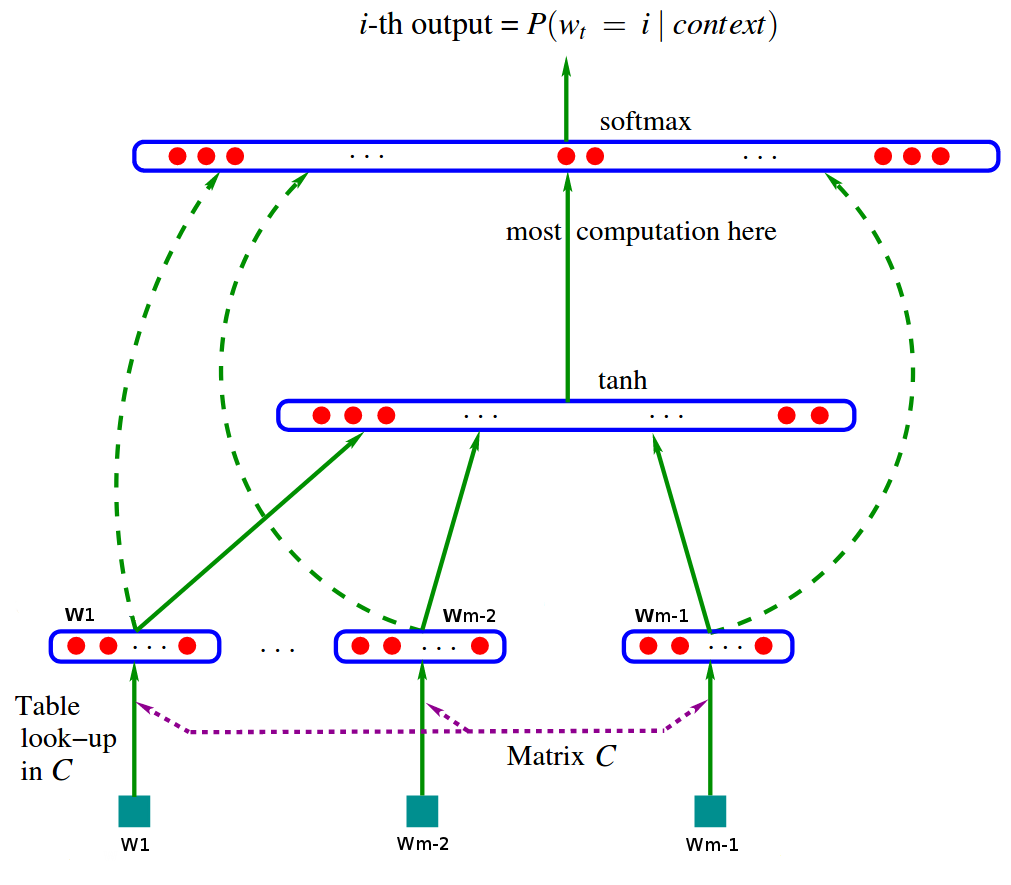
\includegraphics[scale=0.25]{img/bengio_2.png}
    \end{center}
\end{frame}

\begin{frame}{Language Modeling}{Answer f) (2)}
    \begin{itemize}
        \item The proposed architecture was a feed-forward neural network, with
              an embedding layer as input, a single hidden layer with a $tanh$
              activation, and a softmax layer as output.
        \item The input sequence was represented by concatenating all embeddings
              of the given sequence.
        \item The probabilities were computed using a softmax layer, where the
              target was the correct word to predict.
        \item As parameters, let $\mW_w\in \bb{R}^{|V|\times d}$ be the word
              embedding matrix in the input embedding layer,
              $\mW_h\in\bb{R}^{(n\cdot d)\times h}$ be the weight matrix for the
              hidden layer with $n$ being the (max) number of input tokens,
              and $\mW_s\in\bb{R}^{h\times |V|}$ be the weight matrix for the
              softmax layer.
        \item Then, the model was parameterized by
              $\vtheta = \{\mW_w, \mW_h, \mW_s\}$.
    \end{itemize}
\end{frame}

\begin{frame}{Language Modeling}{Question g)}
    \begin{itemize}
        \item What is \emph{self-supervision}? Describe the self-supervised
              training approach used by Bengio et al.\ to train their neural
              language model.
    \end{itemize}
\end{frame}

\begin{frame}{Language Modeling}{Answer g)}
    \begin{itemize}
        \item Self-supervision refers to the process of constructing labeled
              examples by hiding part of an input example and asking the model
              to predict the hidden part given the rest of it.
        \item For images, we can hide part of it and ask the model to predict
              it.
        \item For video, we can ask a model to predict a frame given previous
              $n-1$ frames.
        \item In the context of language models, any sequence of length $n$ in a
              corpus can be used to construct an example for predicting the
              $n$-th word given previous $n-1$ words.
        \item This is what Bengio et al. did.
    \end{itemize}
\end{frame}

\begin{frame}{Language Modeling}{Question h)}
    \begin{itemize}
        \item What problems in n-gram models were no longer an issue with neural
              language models? And what problems still persisted with such
              models?
        \item Explain why the existing limitations are indeed limitations.
    \end{itemize}
\end{frame}

\begin{frame}{Language Modeling}{Answer h)}
    \begin{itemize}
        \item Neural language models such as the one described above did not
              need to store counts of n-grams, thus reducing the memory costs
              significantly.
        \item In addition, the sparsity problem is no longer relevant, as the
              model focuses on observed sequences only.
        \item However, a persisting problem is that the context window is still
              too small, and it can't be enlarged easily in such models.
        \item Why? Note that the input sequence is represented with a vector of
              size $d\cdot n$, where $d$ is the size of the word embeddings and
              $n$ the size of the input sequence.
        \item The hidden layer that takes this vector as input is parameterized
              by $\mW_h\in\set{R}^{(d\cdot n)\times h}$, for input sequence of
              size $n$.
        \item Thus, by increasing the window size, we increase the size of
              $\mW_h$, thus making the model more difficult to train as the
              window grows larger.
        \item And even so, the problem of a fixed window persists.
    \end{itemize}
\end{frame}

\begin{frame}{Language Model Evaluation}{Question a)}
    \begin{itemize}
        \item \textbf{Question:}
              \begin{itemize}
                  \item LMs are often used as part of various
                        \emph{downstream tasks}.
                  \item Give two examples of downstream tasks
                        that may use LMs in their pipeline, and describe how
                        each may use LMs.
              \end{itemize}
              \pause
        \item \textbf{Answer:}
              \begin{itemize}
                  \item Machine translation: a LM may determine which of $n$
                        predicted phrases is more likely.
                  \item Speech recognition: given $n-1$ recognized spoken words,
                        a LM may determine which of a small set of possible
                        words is mostly likely to follow.
                  \item As we can see, LMs are very general tools in NLP.
              \end{itemize}
    \end{itemize}
\end{frame}

\begin{frame}{Language Model Evaluation}{Question b)}
    \begin{itemize}
        \item LMs can be evaluated extrinsically and intrinsically.
              Describe the difference between intrinsic and extrinsic
              evaluation.
        \item Discuss some advantages and disadvantages of each.
    \end{itemize}
\end{frame}

\begin{frame}{Language Model Evaluation}{Answer b)}
    \begin{itemize}
        \item \textbf{Extrinsic:} evaluating model based on performance on a
              specific task, e.g.\ machine translation.
              \begin{itemize}
                  \item This downstream task must use a \emph{downstream} model
                        that uses a language model as part of it, i.e. a machine
                        translation model.
                  \item PROs: we rely on meaningful performance on a task.
                  \item CONs: reported performance dependent on details of
                        task-specific downstream model and evaluation, may not
                        rely so much on language  model performance.
                  \item Also, performance may not translate to different tasks.
              \end{itemize}
        \item \textbf{Intrinsic:} task-neutral evaluation of a model.
              \begin{itemize}
                  \item PROs: no need for possibly expensive downstream
                        pipeline.
                  \item CONs: performance on intrinsic task may not translate to
                        some/all downstream tasks.
              \end{itemize}
    \end{itemize}
\end{frame}

\begin{frame}{Language Model Evaluation}{Question c)}
    \begin{itemize}
        \item \textbf{Question:} Say you are tasked with designing the simplest
              intrinsic evaluation for language models using the basic machine
              learning principle of \emph{held-out data} and a given text
              corpus.
              What sort of evaluation would you propose?
              \pause
        \item \textbf{Answer:} We could split our data into training and test,
              use training data to learn our LM, then evaluate it by computing
              the probability of entire test corpus, i.e. computing the loss
              over by taking the entire test split as a single sequence.
    \end{itemize}
\end{frame}

\begin{frame}{Language Model Evaluation}{Question d)}
    \begin{itemize}
        \item \textbf{Question:}
              \begin{itemize}
                  \item The most common form of intrinsic evaluation of language
                        models is computing its \emph{perplexity} on held-out
                        data.
                  \item Perplexity is defined as follows:
                        \begin{align*}
                            ppl(w_1,w_2,\ldots,w_n) = p(w_1,w2,\ldots,w_n)^{-\frac{1}{n}},
                        \end{align*}
                        where $p$ is the \emph{likelihood} of held-out sequence
                        $x_1, x_2, \ldots, x_n$.
                  \item Describe the intuition of perplexity from the
                        perspective of the likelihood of the data. How does one
                        change when the other changes?
              \end{itemize}
              \pause
        \item \textbf{Answer:} The higher the likelihood, the lower the
              perplexity. Thus, we want to minimize perplexity.
    \end{itemize}
\end{frame}

\begin{frame}{Language Model Evaluation}{Question e)}
    \begin{itemize}
        \item Assume a uniform unigram model over some vocabulary $V$.
        \item What probability does such a model assign to each word in the
              vocabulary?
        \item Compute the likelihood of this model and use it to compute its
              perplexity over a held-out sequence of $n$ words.
    \end{itemize}
\end{frame}

\begin{frame}{Language Model Evaluation}{Answer e) (1)}
    \begin{itemize}
        \item For simplicity, let $V = |V|$.
              Being unigram-based and uniform, this model assigns a probability
              of $\frac{1}{V}$ to each word.
        \item It's likelihood is given by:
              \begin{align*}
                  l(w_1,w_2,\ldots,w_n) & = p(w_1,w_2, \ldots, w_n)     \\
                                        & = p(w_1) p(w_2) \ldots p(w_n) \\
                                        & = \left(\frac{1}{V}\right)^n
                  % & = -n V.
              \end{align*}
              It's perplexity is then:
              \begin{align*}
                  ppl(w_1,w_2,\ldots,w_n) & = l(w_1,w_2,\ldots,w_n)^{-\frac{1}{n}}                   \\
                                          & = \left(\left(\frac{1}{V}\right)^n\right)^{-\frac{1}{n}} \\
                                          & = \left(\frac{1}{V}\right)^{-1}                          \\
                                          & = V.
              \end{align*}
    \end{itemize}
\end{frame}

\begin{frame}{Language Model Evaluation}{Answer e) (2)}
    \begin{itemize}
        \item Thus, the perplexity of LMs is often seen as proportional to the
              size of the vocabulary, where V (the size of the vocabulary) is
              informally seen as an lower-bound for the performance of a model,
              similar to comparing a classifier to a model tnat predicts a
              random class.
        \item In other words, for some vocabulary $V$, if the perplexity of a
              model is greater than $|V|$, we say it performs worse than a
              unigram model that assigns $1/|V|$ probability to each word.
        \item For example, on the \emph{Penn Treebank} dataset, a 5-gram model
              achieves a perplexity of 141, but this can be improved to 80 using
              an RNNs with LSTMs.
        \item In both cases, this is a much lower number that the size of the
              vocabulary.
    \end{itemize}
\end{frame}

\begin{frame}{Recurrent Neural Networks}{Question a)}
    \begin{itemize}
        \item Describe the components of an RNN and discuss how it differs from
              fully-connected neural networks.
        \item What are the parameters of an RNN?
        \item Are RNNs deep? In what way(s)?
    \end{itemize}
\end{frame}

\begin{frame}{Recurrent Neural Networks}{Answer a) (1)}
    \begin{itemize}
        \item RNNs are composed of (possibly parameterized) units that are
              shared across time-steps, i.e.\ across elements of a sequence.
        \item Let's separate these components down into input units, hidden
              units, and output units.
    \end{itemize}
    \vspace{0.5cm}
    \begin{center}
        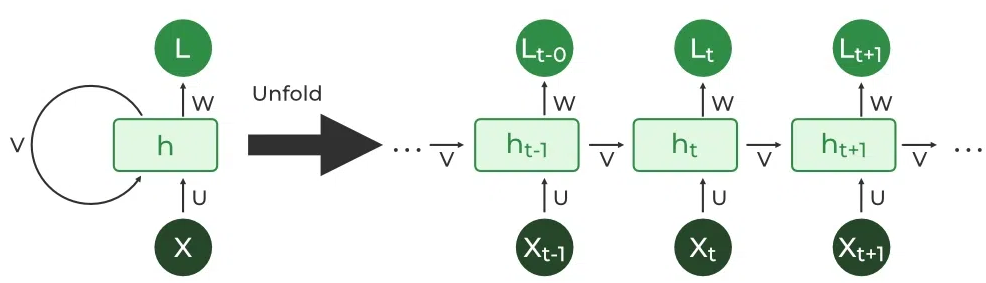
\includegraphics[scale=0.3]{img/rnn_2.png}
    \end{center}
\end{frame}

\begin{frame}{Recurrent Neural Networks}{Answer a) (2)}
    \begin{itemize}
        \item \textbf{Input units:} At time-step $t$, a RNN takes as input
              $\vx_t$, which is a representation of the $t$-th element of a
              given sequence, e.g.\ a word embedding.
              It then transforms it via matrix $\mU$, and passes this
              transformed input to hidden state $\vh_t$.
    \end{itemize}
\end{frame}

\begin{frame}{Recurrent Neural Networks}{Answer a) (3)}
    \begin{itemize}
        \item \textbf{Hidden units:} In addition to the transformed input
              $\vx_t$, a hidden state $\vh_t$ takes as additional input
              $\vh_{t-1}$, i.e.\ the hidden state at previous time-step $t-1$,
              but transformed by matrix $\mV$.
        \item This connection between the same hidden state across time-steps is
              the recurrent connection that gives the network its name (which
              comes from
              \href{https://en.wikipedia.org/wiki/Recurrence_relation}{\underline{recurrent functions}}).
        \item Thus, $\vh_{t}$ takes as input $\mU\vx_t$ and $\mV\vh_{t-1}$,
              combines them via some operation (usually addition), and then
              applies a (possibly non-linear) activation function $f$, before
              passing this result to the hidden state in time-step $t+1$, i.e.\
              $\vh_{t+1}$.
        \item In other words, $\vh_t = f(\mU\vx_t + \mV\vh_{t-1})$.
        \item By sharing parameters $\mU,\mV$ and passing hidden state $\vh_i$
              forward, the intuition is that, at any given time-step $t$,
              $\vh_{t}$ encodes what the model has ``seen'' in the sequence so
              far, i.e.\ all elements up until $t$.
    \end{itemize}
\end{frame}

\begin{frame}{Recurrent Neural Networks}{Answer a) (4)}
    \begin{itemize}
        \item \textbf{Output units:} Optionally, the hidden state may also be
              passed to an output unit $\mL_t$, but transformed via some matrix
              $\mW$ and a (potentially non-linear) activation function $g$.
        \item That is, $\mL_t = g(\mW\vh_t)$.
        \item Whether we have an output unit per time-step or not depends on the
              task at hand (more in the next question).
    \end{itemize}
\end{frame}

\begin{frame}{Recurrent Neural Networks}{Answer a) (5)}
    \begin{itemize}
        \item RNNs are different from FNNs in that they share parameters across
              time-steps, and are thus deep in time.
        \item This is different from fully-connected networks in that those
              typically use different weight matrices in each hidden layer.
        \item However, RNNs can also be stacked to become deep in the same sense
              as fully-connected neural networks.
        \item That is, an RNN layer may produce an output for each input
              element, thus producing an output sequence, which can in turn be
              used as input for another RNN layer.
        \item In such cases, parameters are not shared across layers.
    \end{itemize}
\end{frame}

\begin{frame}{Recurrent Neural Networks}{Question b)}
    \begin{itemize}
        \item How can a RNN be used for a sequence classification task?
        \item And what about for a task where each token in the sequence
              requires a predicted label, e.g.\ part-of-speech (POS) tagging?
        \item Describe the input, output and general architecture of the model.
    \end{itemize}
\end{frame}

\begin{frame}{Recurrent Neural Networks}{Answer b) (1)}
    \begin{itemize}
        \item In \emph{sequence classification}: single prediction per sequence.
        \item E.g.\ in sentiment classification, we may predict
              whether a given sentence describes a positive or negative
              sentiment, i.e.\ binary classification.
        \item Thus, we do not need an output unit per element in the input unit.
              Instead, we may produce a single output input based on the hidden
              state of the final time-step.
        \item This output may be passed by a softmax function to produce a
              relevant probability vector, or for binary classification, a
              logistic function.
    \end{itemize}
    \begin{center}
        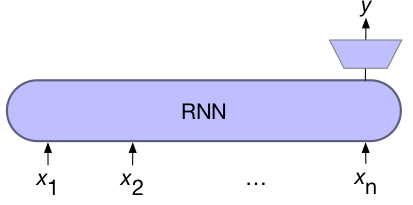
\includegraphics[scale=0.4]{img/sequence_classification_1.png}
    \end{center}
\end{frame}

\begin{frame}{Recurrent Neural Networks}{Answer b) (2)}
    \begin{itemize}
        \item Conversely, requiring a label for each time-step is known as
              \emph{sequence labeling}.
        \item For example, in POS tagging, we want to determine whether each
              word in a sentence is a verb, noun, etc.
        \item Here, the RNN should produce an output at each time-step, as
              illustrated by the image below.
              \begin{center}
                  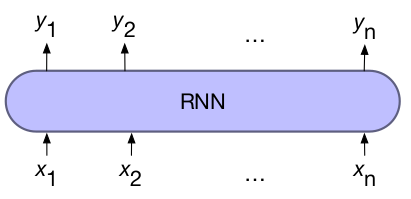
\includegraphics[scale=0.5]{img/sequence_labeling_1.png}
              \end{center}
        \item Each output unit includes softmax function for classification.
        \item In both cases, the inputs and hidden states are as described in
              answer to question (a) above.
    \end{itemize}
\end{frame}

\begin{frame}{Recurrent Neural Networks}{Question c)}
    \begin{itemize}
        \item How can RNNs be used for language modeling? Describe the model's
              architecture.
        \item What is the fundamental problem that RNNs solve over
              fully-connected neural networks for language modeling?
    \end{itemize}
\end{frame}

\begin{frame}{Recurrent Neural Networks}{Answer c) (1)}
    \begin{center}
        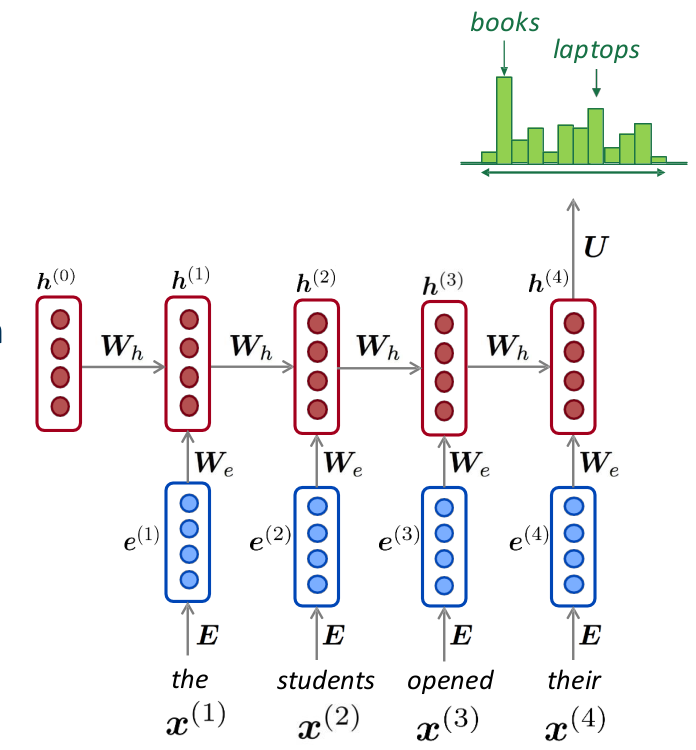
\includegraphics[scale=0.25]{img/lm_rnn_1.png}
    \end{center}
\end{frame}

\begin{frame}{Recurrent Neural Networks}{Answer c) (2)}
    \begin{itemize}
        \item Language models predict the next word given a sequence of $n$
              previous words.
        \item This is done by producing an output at each time-step given the
              corresponding input element and the hidden state at the previous
              time-step.
        \item Thus, unlike LMs implememented with fully-connected networks, such
              as the model from Bengio et al. (2003), here we do not have a
              maximum length of the input sequence that we accept, but can take
              arbitrarily long input sequence.
        \item In addition, unlike n-gram models, predictions made by RNN-based
              language models are not limited by any fixed number of previous
              words, since the hidden state can \emph{in principle} encode all
              the sequence seen so far.
    \end{itemize}
\end{frame}

\begin{frame}{Recurrent Neural Networks}{Question d)}
    \begin{itemize}
        \item What are bidirectional RNNs? What are their advantages and
              disadvantages compared to standard (unidimensional) RNNs?
    \end{itemize}
\end{frame}

\begin{frame}{Recurrent Neural Networks}{Answer d) (1)}
    \begin{center}
        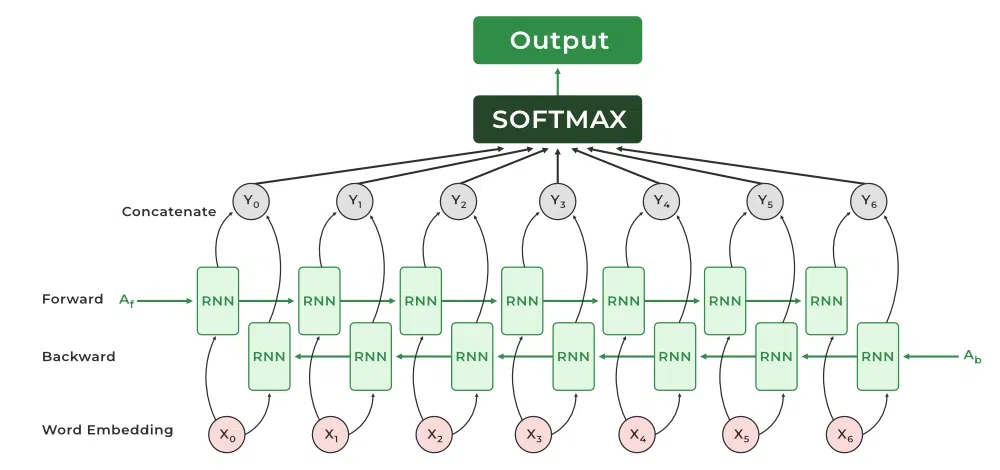
\includegraphics[scale=0.30]{img/Bidirectional-Recurrent-Neural-Network.png}
    \end{center}
    \begin{itemize}
        \item \href{https://www.geeksforgeeks.org/bidirectional-rnns-in-nlp/}{\textcolor{blue}{\underline{Image source}}}
    \end{itemize}
\end{frame}

\begin{frame}{Recurrent Neural Networks}{Answer d) (2)}
    \begin{itemize}
        \item Bidirectional RNNs use an additional hidden state to process a
              given sequence from right to left.
        \item These hidden states are passed ``backward'' from the end of the
              sequence to the beginning, thus encoding it in the opposite
              direction.
        \item This allows the model to, at time-step $t$, encode information
              about both previous and subsequent elements in the input sequence.
        \item Thus, the model has more context to make predictions at any given
              time-step.
        \item A disadvantage is that this is more costly to train, and more
              importantly, such a model cannot be used to make real-time
              predictions, since we do not have information about future
              time-steps.
    \end{itemize}
\end{frame}

\begin{frame}{Recurrent Neural Networks}{Answer d) (3)}
    \begin{itemize}
        \item Perhaps more importantly, isn't it \emph{cheating} to use
              information about future time-steps?
        \item Well, that depends on the application.
        \item If the information is available at inference time, then why not
              use it?
        \item For example, in machine translation, we are usually given an
              entire sequence to translate, so a model can be trained to read
              the entire sequence in both directions before producing a sequence
              in the target language.
        \item This intuition extends to the information we give to any model
              during training, independent of its architecture.
        \item For example, when the goal is to learn generally useful word
              representations, then why not use information in both directions
              to make better use of the context of words in the training set?
        \item This is what the transformer-based model BERT does.
    \end{itemize}
\end{frame}

\begin{frame}{Recurrent Neural Networks}{Answer d) (3)}
    \begin{itemize}
        \item Conversely, when predicting the next word in a sequence, models
              typically have access only to previous words.
        \item Thus, it would not make sense to train models to use information
              about future time-steps to make predictions, as this information
              is not available at inference time.
    \end{itemize}
\end{frame}

\begin{frame}{Recurrent Neural Networks}{Question e)}
    \begin{itemize}
        \item Describe the main problem with RNNs and how LSTMs were designed to
              address this issue.
        \item Give a high-level intuition for each of the gates in an LSTM unit.
    \end{itemize}
\end{frame}

\begin{frame}{Recurrent Neural Networks}{Answer e) (1)}
    \begin{itemize}
        \item The main problem with RNN-based models is that the hiddens state
              needs to encode the entirety of a sequence.
        \item In practice, it's often the case the the hidden states
              ``remembers'' information mostly aobut the most recently seen
              elements, and not those seen far into the past.
        \item This is mostly due to the vanishing gradient problem, which
              describes the impact that operators have over gradient information
              over a long period of time.
        \item Specifically, if an operator makes a gradient smaller, applying
              the same operator multiple times would continuously reduce this
              gradient.
    \end{itemize}
\end{frame}

\begin{frame}{Recurrent Neural Networks}{Answer e) (2)}
    \begin{itemize}
        \item LSTM units were designed to address this issue by allowing the
              model to control what to remember and what to forget about the
              information it has seen.
        \item Thus, models may realize during training that, in order to
              reduce the loss, it's more convenient to retain information
              further in the past instead of more recently seen information.
        \item This is not possible in vanilla RNNs.
        \item LSTM units use parameterized gated mechanisms to allow the model
              to control the flow of information across time-steps.
        \item Specifically, it uses the following gates:
              \begin{itemize}
                  \item \textbf{Forget Gate:} allows model to delete information
                        that it has seen but no longer needs.
                  \item \textbf{Input/Add Gate:} allows model to select what
                        information from the current input and hidden state to
                        use.
                  \item \textbf{Output Gate:} allows the model to separate
                        information needed to produce current output from what
                        is needed to pass to future time-steps.
              \end{itemize}
    \end{itemize}
\end{frame}

\begin{frame}{Recurrent Neural Networks}{Question f)}
    \begin{itemize}
        \item Describe an encoder-decoder architecture and explain how it can be
              used for machine translation, i.e.\ the task of predicting a
              sequence of words in a target language given a sequence of words
              in a source language.
        \item When implementing such an architecture with RNNs, what is the
              input and output of the hidden state in the encoder at each time
              step? And in the decoder?
    \end{itemize}
\end{frame}

\begin{frame}{Recurrent Neural Networks}{Answer f) (1)}
    \begin{itemize}
        \item An encoder-decoder architecture is made up of three components: (i)
              an encoder which takes as input a given source sequence, (ii) a
              context vector produced by the encoder that represents the input
              sequence, and (iii) a decoder, which takes as input the context
              vector and produces an output sequence.
        \item Let's describe the encoder and decoder in more detail.
    \end{itemize}
\end{frame}

\begin{frame}{Recurrent Neural Networks}{Answer f) (2)}
    \begin{itemize}
        \item \textbf{Encoder:} In machine translation, the encoder takes as
              input the source sequence, and produces a context vector (usually
              the hidden state of the last time-step).
        \item This encoder produces no other outputs and in general can be any
              architecture that makes as much use of the input data as possible.
        \item RNN-based encoders are typically stacked bidirectional RNNs with
              LSTM units (biLSTMs for short), but this can also be done with
              other types of architectures, e.g.\ transformers.
    \end{itemize}
\end{frame}

\begin{frame}{Recurrent Neural Networks}{Answer f) (3)}
    \begin{itemize}
        \item \textbf{Decoder:} The decoder takes as input the context vector
              and a ``beginning of sentence'' tag (in machine translation, this
              tag is used to separate source from target sentences pairs shown
              to the model).
        \item Using this, it produces a hidden state and an output word,
              \emph{both of which} are then used as input for the hidden state
              of the decoder in the next time step.
        \item In addition, it's common to use the context vector produced by
              the encoder as input in each time-step of the decoder, to preserve
              this information.
    \end{itemize}
\end{frame}

\begin{frame}{Recurrent Neural Networks}{Answer f) (4)}
    \begin{itemize}
        \item Formally, the hidden state of the decoder at time-step $t$ is
              given by:
              \begin{align*}
                  \vh_t^d & = g(\vy_{t-1},\vh_{t-1}^d,\vc),
              \end{align*}
              where $\vy_{t-1}$ is the embedding of word produce by decoder in
              the previous time-step, and $\vc$ is the context vector produced
              by the encoder.
        \item This decoder architecture is illustrated in the image below.
              \begin{center}
                  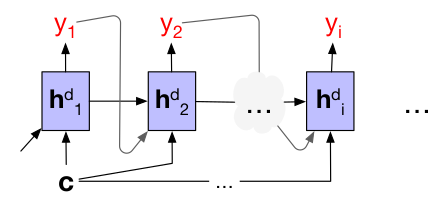
\includegraphics[scale=0.5]{img/encoder_decoder_for_mt_1.png}
              \end{center}
    \end{itemize}
\end{frame}

\begin{frame}{Sampling for Text Generation}{Context}
    \begin{itemize}
        \item An important aspect of using language models to (autoregressively)
              generate text is the step of \emph{sampling} the next word from
              the distribution over words in our vocabulary that is produced by
              a language model.
        \item In this task, we discuss some basic methods for sampling from this
              distribution to generate text.
    \end{itemize}
\end{frame}

\begin{frame}{Sampling for Text Generation}{Question a)}
    \begin{itemize}
        \item What is autoregressive text generation?
        \item What are its advantages compared non-autoregressive text
              generation?
        \item And its disadvantages?
    \end{itemize}
\end{frame}

\begin{frame}{Sampling for Text Generation}{Answer a)}
    \begin{itemize}
        \item \textbf{Autoregressive generation:} generate sequence of
              word/tokens by repeatedly sampling the next word/token
              conditioned on previously chosen words/tokens.
              \pause
        \item \textbf{Advantages:} can capture dependencies between
              words/tokens in a sequence.
              \pause
        \item \textbf{Disadvantages:} can be slow to generate long
              sequences, the longer the range of dependencies that need
              to be captured, the higher the cost of sampling.
              In other words, non-autoregressive generation is
              cheaper/faster.
    \end{itemize}
\end{frame}

\begin{frame}{Sampling for Text Generation}{Question b)}
    \begin{itemize}
        \item In a machine translation setting, let
              $X = \{x_1, x_2, \ldots, x_n\}$ be the input sequence in some
              source language, $Y = \{y_1, y_2, \ldots, y_m\}$ the output
              sequence in some target language, and $p(y_t|X,\vtheta)$ the
              distribution for the $t$-th word in a non-autoregressive setting
              using a model parameterized by $\vtheta$.
        \item Give the corresponding expression for $p$ in an autoregressive
              model.
              \pause
        \item \textbf{Answer:}$p(y_t|y_{<t},X,\theta)$
    \end{itemize}
\end{frame}

\begin{frame}{Sampling for Text Generation}{Question c)}
    \begin{itemize}
        \item Let $\operatorname{sample}(p)$ be a function to sample a word
              from the autoregressive expression for $p$ you provided in the
              previous question, and $<s>, </s>$ be the start-of-sentence and
              end-of-sequence tokens, respectively.
        \item Write an algorithm in pseudocode to autoregressively generate a
              sequence of words of arbitrary length.
    \end{itemize}
\end{frame}

\begin{frame}{Sampling for Text Generation}{Answer c)}
    \begin{algorithmic}
        %   \STATE $i \leftarrow 1$
        \STATE $w \leftarrow \operatorname{sample}(p(w_i|<s>))$
        \STATE out $\leftarrow [w]$
        \WHILE{$w \neq </s>$}
        %   \STATE $i \leftarrow i + 1$
        \STATE $w \leftarrow \operatorname{sample}(p(w_i|out))$
        \STATE out $\leftarrow$ out $+ [w]$
        \ENDWHILE
        \RETURN out
    \end{algorithmic}
\end{frame}

\begin{frame}{Sampling for Text Generation}{Question c)}
    \begin{itemize}
        \item The most straightforward way to implement the \emph{sample}
              function used in the previous question is by choosing the word
              with the highest probability.
        \item This is known as \textbf{greedy sampling}.
        \item Can you think of advantages and disadvantages to such an approach?
        \item Use the following two incomplete sentences to reason about this.
              \begin{enumerate}
                  \item The capital of Germany is $\ldots$
                  \item The title of my talk is $\ldots$
              \end{enumerate}
    \end{itemize}
\end{frame}

\begin{frame}{Sampling for Text Generation}{Question c)}
    \begin{itemize}
        \item \textbf{Advantages:} straightforward to understand/implement.
        \item \textbf{Important disadvantage:} can lead to generation of text
              that is predictable and repetitive.
        \item In fact, given a model and the same input sequence, greedy
              sampling should deterministically produce the same output
              sequence.
        \item This is convenient when we want to predict facts that do not
              change, e.g.\ the answer to ``What is the capital of Germany''?
        \item But this is an undesired property when we want to generate text
              that is more original/creative, such as what should follow after
              ``The title of my talk is''
    \end{itemize}
\end{frame}

\begin{frame}{Sampling for Text Generation}{Question d)}
    \begin{itemize}
        \item Another way to implement the \emph{sample} function is by
              \textbf{randomly sampling} from $p$.
        \item This means we sample a word $w$ with probability $p(w)$, so that
              words with higher probability get sampled more often, while words
              with lower probability get sampled less often.
        \item Can you think of advantages and disadvantages to such an approach?
        \item \textbf{Hint:} the size of the vocabulary is often very large, and
              for a given input sequence, the distribution over words is very
              skewed.
    \end{itemize}
\end{frame}

\begin{frame}{Sampling for Text Generation}{Answer d)}
    \begin{itemize}
        \item Random sampling can lead to more diverse and creative text, as it
              allows the model to sample from the entire vocabulary.
        \item However, it can also lead to less coherent text, as the model may
              sample words that are less likely to follow the previous words.
        \item In addition, the size of the vocabulary is often very large, and
              for a given input sequence, the distribution over words is very
              skewed.
        \item This means that the model may sample from words that are very
              rare, and thus produce text that is less coherent.
    \end{itemize}
\end{frame}

\begin{frame}{Sampling for Text Generation}{Question e)}
    \begin{itemize}
        \item Can you think of an approach that can be used to sample from the
              distribution over words in a more balanced way compared to both
              \emph{greedy} and \emph{random} sampling?
        \item What are its advantages and disadvantages compared to the
              approaches described in the previous questions?
    \end{itemize}
\end{frame}

\begin{frame}{Sampling for Text Generation}{Answer e) (1)}
    \begin{itemize}
        \item The answer is \textbf{top-k sampling}. \
        \item This is a generalization of \emph{greedy} sampling, where we now
              sample from the set of $k$ words with the most probability.
        \item When $k=1$, we have greedy sampling.
        \item When $k=|V|$, we have random sampling.
        \item Generally, for values of $k > 1$, we allow the model to generate
              words that are not so predictible, but still probable enough that
              the resulting text can be of high-quality.
        \item \textbf{Important disadvantage:} $k$ is a fixed value, but the
              distributions over words produced by a model change for given
              inputs.
        \item E.g.\ when the input sequence is ``The capital of Germany is'',
              most of the probability mass in the resulting distribution would
              ideally be in the Berlin token (or combination of tokens),
              which is a (proper) noun.
    \end{itemize}
\end{frame}

\begin{frame}{Sampling for Text Generation}{Answer e) (2)}
    \begin{itemize}
        \item But when the input sequence is ``The title of my talk'', the
              probability mass would most likely be in the token ``is'' or
              similar verbs.
        \item To address this issue, \textbf{top-p sampling} was proposed, where
              we sample from the words that add up to the top $p$ probability
              mass in the distribution.
        \item That way, we can sample from a variable number of words given
              different input sequences.
        \item A good model may indeed learn to put most of the mass in the
              answer to a factual question, e.g. Berlin is the capital of
              Germany, or more generally distribute it more evenly among several
              probable words in other settings.
    \end{itemize}
\end{frame}

\begin{frame}{Sampling for Text Generation}{Question f)}
    \begin{itemize}
        \item \emph{Temperature} sampling is another approach, where instead of
              truncating a model distribution, we reshape it.
        \item It is defined in the context of softmax distributions as follows:
              \begin{align*}
                  \vy = \operatorname{softmax}\left(\frac{\vu}{\tau}\right),
              \end{align*}
              where $\vu$ is the unnormalized distribution over words, i.e.\
              a vector of logits, $\tau$ is the temperature parameter, and we do
              an element-wise division with it.
        \item Describe the impact that different values of $\tau$ have over the
              resulting model distribution that we will then use to sample the
              next word from.
        \item Specifically, how does the distribution change as $\tau$ is less
              than 1 and approaches zero? And as it approaches infinity?
    \end{itemize}
\end{frame}

\begin{frame}{Sampling for Text Generation}{Answer f)}
    \begin{itemize}
        \item As $tau$ approaches zero and is less than 1, it will increase the
              values of all logits, e.g.\ $12 < 12/0.5 < 12/0.3$.
        \item This will result in increased probability mass on words that
              already have high mass, and decreased probability mass on words
              that had low mass in the first place.
        \item Thus, as we decrease the temperature, most of the probability mass
              in the distribution concentrates around the most probable words.
        \item Conversely, if we increase the temperature to values greater than
              1 and beyond, the probability mass will be more evenly distributed
              across all words, as the operation will decrease values of all
              logits.
        \item See some animations
              \href{https://medium.com/@harshit158/softmax-temperature-5492e4007f71}{\textcolor{blue}{\underline{here}}}.
    \end{itemize}
\end{frame}

\end{document}
